%!TEX root = /Users/dbreuer/Documents/Work/_FH/_Master/master_thesis/Main/Master Thesis.tex

\chapter{Prototypische Realisierung} % (fold)
\label{cha:prototypische_realisierung}

  Nachdem in das COSIMA-Projekt eingeführt und ein Szenario beschrieben wurde, dass zur Validierung der bisherigen Architektur dienen soll wird in dem vorliegenden Kapitel die prototypische Realisierung der Architektur und des beschriebenen Szenario.
  
  Die Implementierung ist dabei in der Programmiersprache Java in Version 5.0 vorgenommen worden und erfolgte in zwei, von einander abhängigen Stufen:
  
  \begin{enumerate}
    \item Prototypische Realisierung der wesentlichen Architekturmerkmale und
    \item Implementierung des in \ref{sub:das_anwendungsszenario} beschriebenen Szenario auf Basis der Architektur.
  \end{enumerate}
  
  Im ersten Abschnitt dieses Kapitel wird daher zunächst das Vorgehen und Ergebnis bei der Umsetzung der Architektur beschrieben. Im Anschluss daran findet sich eine Erläuterung zur Implementierung des Szenario. Die Validierung und deren Ergebnisse werden im Anschluss in Kapitel \ref{cha:validierung_der_architektur} dargelegt.

% - Vorgehen bei der Realisierung erläutern
% - Kurz (!!) auf das Santiago Projekt eingehen (da es im allerersten Schritt dazu gedient hat, eine erste funktionierende Grundlage der Architektur zu schaffen)
% - Wichtige Punkte herausarbeiten
% - Auf Implementierungsdetails nur an grundlegenden Stellen eingehen
% - Schwierigkeiten und vor allem deren Problemlösungen darstellen
% - Auswirkungen dieser Probleme/Lösungen für die Architektur
% - Fokus vor allem im Text auf das Vorgehen und Wendepunkte
% - Hauptteil der Quellcode
% - Funktionierenden Code mit Build Tool und Dokumentation ausliefern (!!)

\section{Realisierung der Architektur} % (fold)
\label{sec:realisierung_der_architektur}

  Bevor eine Anwendung auf Basis einer Architektur oder eines Rahmenwerk entwickelt werden kann, muss im ersten Schritt die Architektur oder das Rahmenwerk selbst existieren. In~\citep{handbuch_der_software_architektur} wird beschrieben, dass bei der Entwicklung bei Rahmenwerken in der Regel zuvor eine Reihe von ähnlichen Anwendungen entstehen, aus denen dann die Gemeinsamkeiten in ein Rahmenwerk extrahiert werden. Da es sich bei COSIMA zum Teil auch um ein Rahmenwerk handelt ($\to$ \ref{sub:framework_oder_architektur}) hätte bei der Entwicklung entsprechend verfahren werden können. Auf Grund der beschrieben Neuartigkeit des Projekts musste jedoch auf bereits in Abschnitt \ref{cha:szenario} Eingangs beschriebene szenariobasierte Vorgehen zurückgegriffen werden.
  
  Bei der konkreten Implementierung der Architektur hingegen wurde sich wieder für einen stärker \emph{bottom-up} getriebenen Ansatz entschieden. Ziel war es einen abgegrenzten Anwendungsfall mit der entworfenen Architektur umzusetzen. Anschließend ließe sich, in der so entstandenen Architekturimplementierung das eigentliche Szenario realisieren.
  
  Dieser Anwendungsfall ist in Abbildung \ref{fig:images_Santiago_Anwendungsfall} schematisch dargestellt. Trotz seiner Einfachheit beinhaltet der Anwendungsfall die wesentlichen Elemente, die zur Extraktion den grundsätzlichen Funktionalitäten der Architektur notwendig waren\footnote{Aufgrund der leichteren sprachlichen Trennung erhielt dieser Anwendungsfall den Codenamen \emph{Santiago}, der weiteren Verlauf synomym zu diesem Anwendungsfall verwandt werden soll.}:
  
  \begin{figure}[ht]
    \centering
      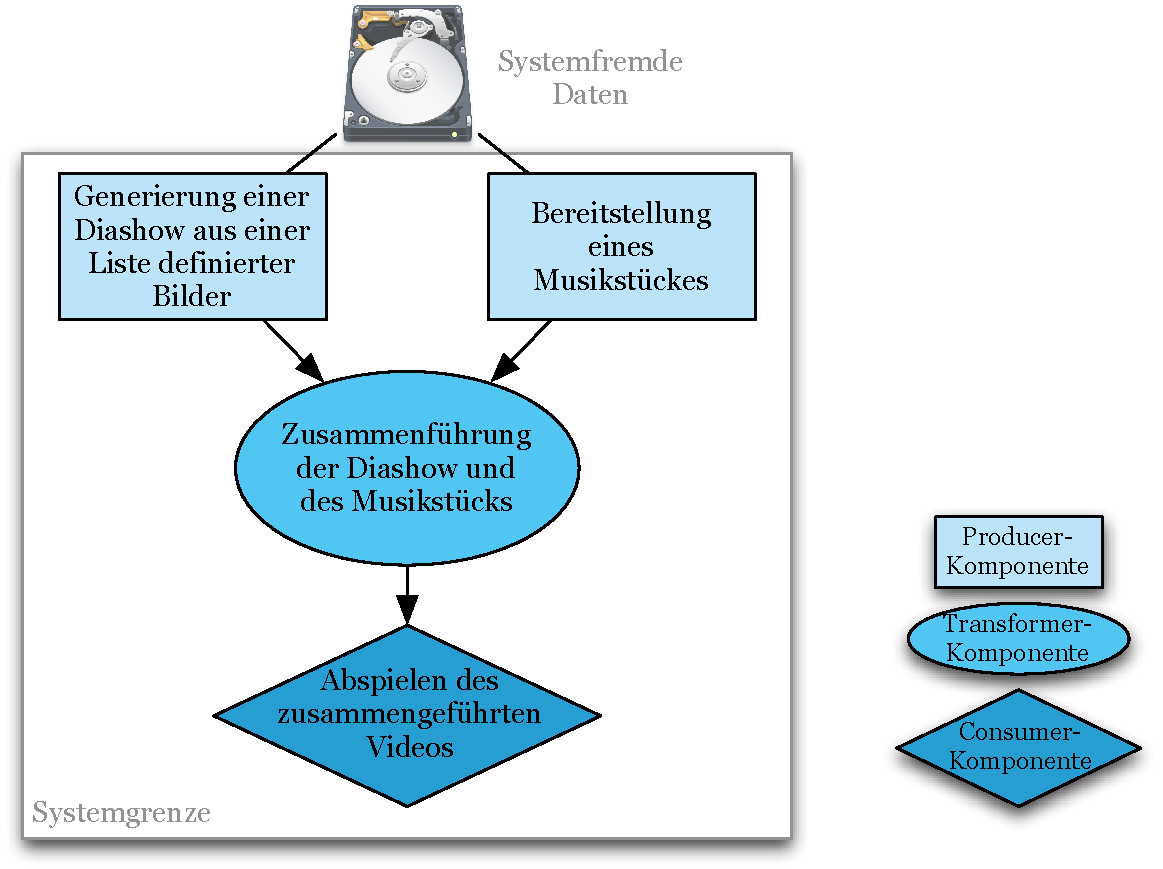
\includegraphics[width=.9\textwidth]{images/Santiago_Anwendungsfall.pdf}
    \caption{Anwendungsfall für die Realisierung der Architektur}
    \label{fig:images_Santiago_Anwendungsfall}
  \end{figure}

  \begin{itemize}
    \item Verarbeitung von unterschiedlichen Medien
    \item Umsetzung der einzelnen Verarbeitungsschritte in dedizierten Komponenten
    \item Anordnung dieser Komponenten nach dem Quelle-Komponente-Senke Prinzip
  \end{itemize}

  Wie aus diesen wenigen einfachen Eigenschaften die wesentlichen Merkmale von COSIMA extrahiert wurden, behandelt der nächste Abschnitt.

  % TODO: Klären ob diese Punkte noch eingearbeitet werden müssen.
  % 
  % Beschreibung der Workflow Komponente. Vor allem Begründung warum selber gebaut -> Handelt es sich um Geschäftsprozesse? Dafür Prozess und Workflow definieren und auch auf Samma's Arbeit verweisen. Möglichkeiten zur Verwendung von BPEL aufzeigen.
  % 
  % Während der iterativen Entwicklung dieser Anwendung wurde sie sukzessive um die einzelnen Elemente und deren Funktionalitäten der COSIMA-Architektur ergänzt.
  % 
  % ZUR SERVICEKOMPOSITION: Aus den in~\ref{sub:service_komposition} genannten Gründen kann auch bei der prototypische Realisierung auf die Verwendung einer existierenden Prozessbeschreibungssprache verzichtet werden.
  
\subsection{Vorgehen} % (fold)
\label{sub:vorgehen_architektur}

  Die Entwicklung der beschriebenen Anwendung und die anschließende Extraktion und Refaktorisierung hin zu einer Anwendung, die innerhalb von COSIMA realisiert ist, erfolgte in einem iterativen Vorgehen. Im ersten Schritt wurden die vier einzelnen Komponenten mit ihren jeweiligen Funktionalitäten implementiert. Die Ausführung dieser Komponenten übernimmt ein einfaches \verb!Main!-Programm (Listing \ref{lst:santiago_plain}), dass die notwendigen Parameter dabei direkt übergibt.

\lstinputlisting[caption=\texttt{SantiagoPlain}-Klasse zur einfachen Ausführung des Anwendungsfalls,label=lst:santiago_plain,language=Java,firstline=11,morekeywords={[2]VideoPlayer,SlideshowGenerator,MusicOMat}]{../code/Santiago/src/main/java/de/fhkoeln/santiago/codesamples/SantiagoPlain.java}

  Die rot markierten Klassen stellen die Implementierungen der einzelnen Operationen dar. Die Umsetzung als Klassenmethoden ist jedoch nicht für den Einsatz in einer verteilten Umgebung geeignet. Eine parallele Verwendung der selben Komponente wäre so nur schwer umsetzbar. Daher mussten im nächsten Schritt die Operationen jeweils auf Instanzen der Komponenten durchgeführt werden. Da alle Komponenten zwei wesentliche Gemeinsamkeiten aufweisen, \emph{a)} Die Übergabe von Eingabeparametern und \emph{b)} Die Ausführung der Operation unter Berücksichtigung dieser Parameter, lag die Einführung einer Oberklasse nahe. Die entsprechenden Klassen erbten in der nächsten Iteration daher von der abstrakten Klasse \verb!AbstractComponent! (siehe Listing \ref{lst:abstract_component_simple_class}). Sie definiert die beiden Methoden \verb!setInput(String [] inputs)! und \verb!execute()!.

  \lstinputlisting[caption=Einfache \texttt{AbstractComponent}-Klasse,label=lst:abstract_component_simple_class,language=Java,firstline=8,morekeywords={[3]execute,getInput,setInput}]{../code/Santiago/src/main/java/de/fhkoeln/santiago/codesamples/AbstractComponent.java}
  
  Das ausführende Programm aus Listing \ref{lst:santiago_plain} kann nun die generalisierten Komponenten mit ihrer homogenen Schnittstelle verwenden um die Operationen durchzuführen. Die Änderungen der Anwendung sind in Listing \ref{lst:santiago_plain_with_general_components} dargestellt. Als eine erste Abstraktion der Parameter dient in diesem Fall noch ein primitives String-Array, im weiteren Verlauf wird daraus ein vollständiges \emph{Value-Object}~\citep[S. 486]{fowler03peaa} entstehen. Die Implementierung der \verb!execute()!-Methode ist nach dem \emph{Template Method} Entwurfsmuster vorgenommen worden~\citep[325]{design_patterns}\footnote{In späteren Iterationen lassen sich so leicht Funktionalitäten hinzufügen, die vor oder nach der eigentlichen Operation durchgeführt werden müssen.}.

  \lstinputlisting[caption=Erweitertes Santiago Programm mit generalisierten Komponenten,label=lst:santiago_plain_with_general_components,language=Java,firstline=21,lastline=34,morekeywords={[3]AbstractComponent}]{../code/Santiago/src/main/java/de/fhkoeln/santiago/codesamples/SantiagoPlainWithGeneralComponents.java}
  
  Innerhalb einer COSIMA-Anwendung kann eine Transformer-Komponente nur Mediendaten verarbeiten, die bereits im System vorhanden sind, also über den Medien Broker abgerufen werden können. Für den aktuellen Anwendungsfall bedeutet das, was bereits in Abbildung \ref{fig:schema_des_anwendungsszenario} dargestellt wurde: Eine Producer-Komponente muss das Musikstück erst innerhalb der Systemgrenzen \emph{bekannt machen}. In dem Kontext von COSIMA hat das die Bedeutung, dass ein Medienobjekt erzeugt und über den Medien Broker bereitgestellt wird. Die Einbindung dieser zusätzlichen Komponente ist in Listing \ref{lst:santiago_plain_with_music_provider} zu sehen.
  
  \lstinputlisting[caption=Integration einer dedizierter Komponente zur Bereitstellung der Musik,label=lst:santiago_plain_with_music_provider,language=Java,firstline=21,lastline=24,morekeywords={[3]MusicProvider}]{../code/Santiago/src/main/java/de/fhkoeln/santiago/codesamples/SantiagoPlainWithMusicProvider.java}
  
  
  
  
  % -----------------
  
  

 Offensichtlich müssen die rot markierten Klassen weiter bearbeitet werden, hin zu Komponenten. Aber auch \verb!musicPath! und \verb!imagePath! müssen als externe Daten weiter abstrahiert werden. Einführung einer systeminternen Komponente, die die Musikdaten bereitstellt!
 
 Dafür folgende Schritte notwendig:
 
 - Definition einer Schnittstelle für Ausführung der Funktionalität\\
 - Einführung eines Value-Objects, zum Handling der Ein- und Ausgabedaten
 
  Anschließend Möglichkeit zur abstrakten (deklarativen) Definition der Ausführung notwendig (Workflow-Definition). Für den Prototypen wurde eine einfache Lösung selbst implementiert. Ermöglicht einen besseren Einblick in die Anforderungen und besseres Verständnis im Rahmen der Validierung. Verwendung einer etablierten Lösung wie BPEL hätte eine zusätzliche Komplexität eingeführt, die nicht zur Zielerreichung beigesteuert hätte (vgl. Umfang bei~\citep{samma08}). Auch ist keine zustandbasierte Lösung implementiert worden, wie sie bei~\citep{biornstad2006cfs} vorgeschlagen (und auch von BPEL implementiert). Grund: Ohnehin nur Prototyp, Inhalt weiterer Arbeiten.
  
\begin{lstlisting}[caption=\texttt{WorkflowDefinition}-Schnittstelle,label=lst:workflow_definition_interface]
package de.fhkoeln.cosima.workflow;
/**
 * The Interface for accessing a workflow definition from an executing instance.
 */
public interface WorkflowDefinition {
  /**
   * @return The Set of those Elements which need to proccessed next.
   */
  public Set<WorkflowElement> getNextElements() throws NoSuchElementException;
  /**
   * @return The amount of Workflow Elements.
   */
  public int size();
  /**
   * Rewinds the definition list, so it can be read again.
   */
  public void rewind();
  /**
   * @return If there are any more elements to fetch or not.
   */
  public boolean hasNextElements();
}
\end{lstlisting}

% subsection vorgehen_architektur (end)
  
\subsection{Probleme und Lösungen} % (fold)
\label{sub:probleme_und_loesungen_architektur}

  - Welche Probleme sind aufgetaucht?
  - Wie wurden diese gelöst?
  - Auswirkungen auf die Architektur!
  - Workflow ohne externes Messaging System möglich!?

% subsection probleme_und_loesungen_architektur (end)

% section realisierung_der_architektur (end)

\section{Realisierung des Szenario} % (fold)
\label{sec:realisierung_des_szenario}

  - Nerstrand Projekt
  - wichtige Punkte beschreiben
  - top-down Ansatz

\subsection{Extrahierte Anforderungen} % (fold)
\label{sub:extrahierte_anforderungen}

% subsection extrahierte_anforderungen (end)

\subsection{Vorgehen} % (fold)
\label{sub:vorgehen_szenario}

  - wie wurde bei der Umsetzung des Anwendungsszenario vorgegangen?

% subsection vorgehen_szenario (end)

\subsection{Probleme und Lösungen} % (fold)
\label{sub:probleme_und_loesungen_szenario}

  - Welche Probleme sind aufgetaucht?
  - Wie wurden diese gelöst?
  - Auswirkungen auf die Architektur!

% subsection probleme_und_loesungen_szenario (end)

% section realisierung_des_szenario (end)

% chapter prototypische_realisierung (end)